\begin{figure}[h!]
    \centering
    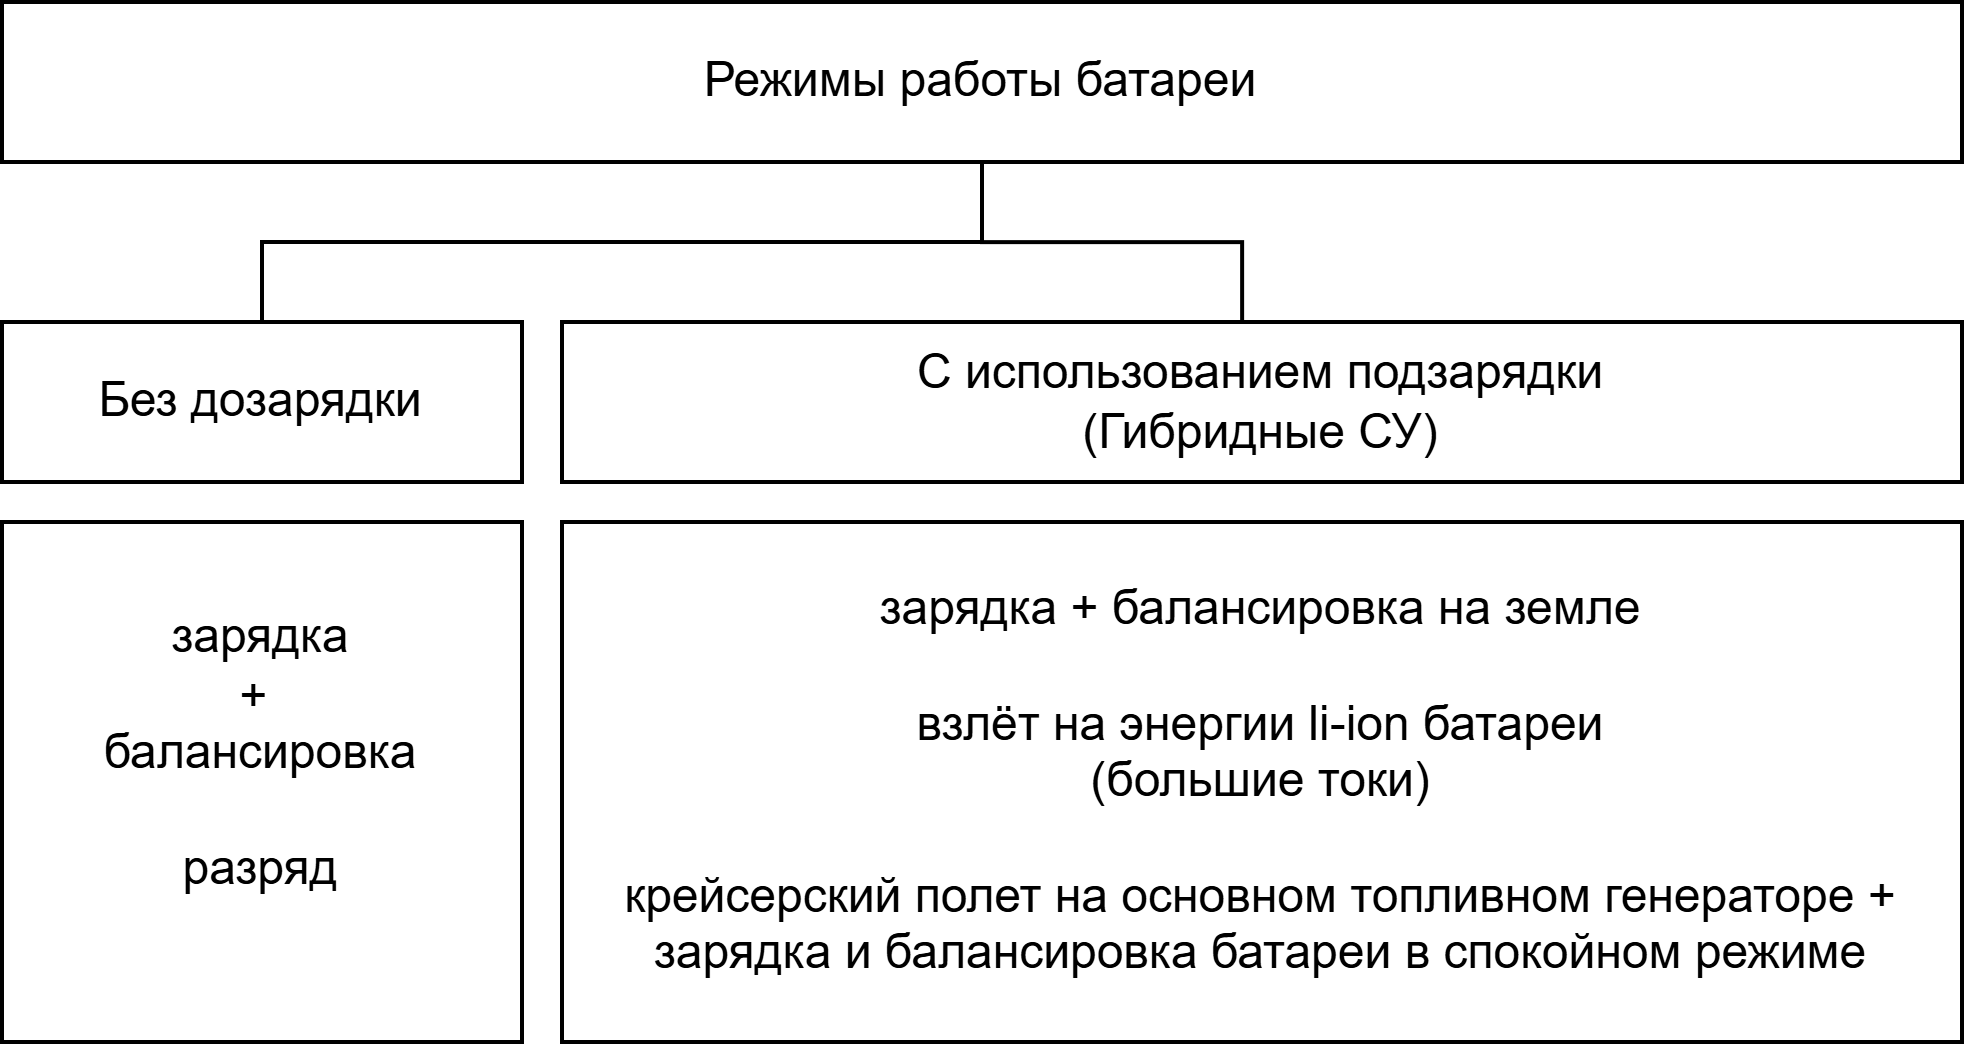
\includegraphics[width=0.9\linewidth]{img/battery_work_modes.png}
    \caption{Схема возможных режимов работы системы "батарея-нагрузка" в \acs{la}}
    \label{fig:mods_li_ion}
\end{figure}

Балансировка может производиться при разных обстоятельствах, режимы работы батареи смогут быть разными, а именно:
\begin{enumerate}[noitemsep, topsep=0pt, partopsep=0pt]
    \item Зарядка и балансировка до начала эксплуатации \acs{la}.
    \item Балансировка в простое (возможно только для активной \acs{bms}).
    \item Балансировка при активном использовании батареи.
\end{enumerate}
Стоит отметить, что в последнем случае балансировка может оказаться бесполезной, 
поскольку балансировочные токи должны быть порядка скорости разбалансировки ячеек,
что не всегда возможно, т.к. поглощение тока ячейками ограничено, как и максимальный балансировочный ток \acs{bms}. 
